%%%%%%%%%%%%%%%%%%%%%%%%%%%%%%%%%%%%%%%%%
% Beamer Presentation
% LaTeX Template
% Version 1.0 (10/11/12)
%
% This template has been downloaded from:
% http://www.LaTeXTemplates.com
%
% License:
% CC BY-NC-SA 3.0 (http://creativecommons.org/licenses/by-nc-sa/3.0/)
%
%%%%%%%%%%%%%%%%%%%%%%%%%%%%%%%%%%%%%%%%%

%----------------------------------------------------------------------------------------
%	PACKAGES AND THEMES
%----------------------------------------------------------------------------------------

\documentclass[handout]{beamer}

\mode<presentation> {

% The Beamer class comes with a number of default slide themes
% which change the colors and layouts of slides. Below this is a list
% of all the themes, uncomment each in turn to see what they look like.

%\usetheme{default}
%\usetheme{AnnArbor}
%\usetheme{Antibes}
%\usetheme{Bergen}
%\usetheme{Berkeley}
%\usetheme{Berlin}
%\usetheme{Boadilla}
%\usetheme{CambridgeUS}
%\usetheme{Copenhagen}
%\usetheme{Darmstadt}
%\usetheme{Dresden}
%\usetheme{Frankfurt}
%\usetheme{Goettingen}
%\usetheme{Hannover}
%\usetheme{Ilmenau}
%\usetheme{JuanLesPins}
%\usetheme{Luebeck}
\usetheme{Madrid}
%\usetheme{Malmoe}
%\usetheme{Marburg}
%\usetheme{Montpellier}
%\usetheme{PaloAlto}
%\usetheme{Pittsburgh}
%\usetheme{Rochester}
%\usetheme{Singapore}
%\usetheme{Szeged}
%\usetheme{Warsaw}

% As well as themes, the Beamer class has a number of color themes
% for any slide theme. Uncomment each of these in turn to see how it
% changes the colors of your current slide theme.

%\usecolortheme{albatross}
%\usecolortheme{beaver}
%\usecolortheme{beetle}
%\usecolortheme{crane}
%\usecolortheme{dolphin}
%\usecolortheme{dove}
%\usecolortheme{fly}
%\usecolortheme{lily}
%\usecolortheme{orchid}
%\usecolortheme{rose}
%\usecolortheme{seagull}
%\usecolortheme{seahorse}
%\usecolortheme{whale}
%\usecolortheme{wolverine}

%\setbeamertemplate{footline} % To remove the footer line in all slides uncomment this line
%\setbeamertemplate{footline}[page number] % To replace the footer line in all slides with a simple slide count uncomment this line

%\setbeamertemplate{navigation symbols}{} % To remove the navigation symbols from the bottom of all slides uncomment this line
}

\usepackage{graphicx} % Allows including images
\usepackage{booktabs} % Allows the use of \toprule, \midrule and \bottomrule in tables
\usepackage{cool}
\usepackage{amsmath}
\usepackage{amssymb}
\usepackage{bm}
\usepackage{physics}
\usepackage{hyperref}
\usepackage{listings}

\newcommand{\prob}{\mathcal{P}}
\newcommand{\rew}{\mathcal{R}}
\newcommand{\states}{\mathcal{S}}
\newcommand{\actions}{\mathcal{S}}

\DeclareMathOperator*{\argmin}{arg\,min}
\DeclareMathOperator*{\argmax}{arg\,max}

\newcommand{\bvpi}{\bm{V}^{\pi}}
\newcommand{\bvs}{\bm{V}^*}
\newcommand{\bbpi}{\bm{B}^{\pi}}
\newcommand{\bbs}{\bm{B}^*}
\newcommand{\bv}{\bm{V}}

%----------------------------------------------------------------------------------------
%	TITLE PAGE
%----------------------------------------------------------------------------------------

\title[Dynamic Programming Chapter]{A Guided Tour of \href{http://stanford.edu/~ashlearn/RLForFinanceBook/book.pdf}{\underline{\textcolor{yellow}{Chapter 3}}}: \\  Dynamic Programming} % The short title appears at the bottom of every slide, the full title is only on the title page

\author{Ashwin Rao} % Your name
\institute[Stanford] % Your institution as it will appear on the bottom of every slide, may be shorthand to save space
{ICME, Stanford University
 % Your institution for the title page
}

\date % Date, can be changed to a custom date

\begin{document}
\lstset{language=Python}  
\begin{frame}
\titlepage % Print the title page as the first slide
\end{frame}

% \begin{frame}
% \frametitle{Overview} % Table of contents slide, comment this block out to remove it
% \tableofcontents % Throughout your presentation, if you choose to use \section{} and \subsection{} commands, these will automatically be printed on this slide as an overview of your presentation
% \end{frame}

\begin{frame}
\frametitle{Dynamic Programming for Prediction and Control}
\pause
\begin{itemize}[<+->]
\item Prediction: Compute the Value Function of an MRP
\item Control: Compute the Optimal Value Function of an MDP
\item (Optimal Policy can be extracted from Optimal Value Function)
\item Planning versus Learning: access to the $\mathcal{P}_R$ function (``model'')
\item Original use of {\em DP} term: MDP Theory {\em and} solution methods
\item Bellman refered to DP as the {\em Principle of Optimality}
\item Later, the usage of the term DP diffused out to other algorithms
\item In CS, it means "recursive algorithms with overlapping subproblems"
\item We restrict the term DP to: "Algorithms for Prediction and Control"
\item Specifically applied to the setting of \lstinline{FiniteMarkovDecisionProcess}
\item Later we cover extensions such as Asynchronous DP, Approximate DP
\end{itemize}
\end{frame}

\begin{frame}
\frametitle{Solving the Value Function as a {\em Fixed-Point}}
\pause
\begin{itemize}[<+->]
\item We will be covering 3 Dynamic Programming algorithms
\item Each of the 3 algorithms is founded on the Bellman Equations
\item Each is an iterative algorithm converging to the true Value Function
\item Each algorithm is based on the concept of {\em Fixed-Point}
\begin{definition}
The Fixed-Point of a function $f: \mathcal{D} \rightarrow \mathcal{D}$ (for some arbitrary domain $\mathcal{D}$) is a value $x \in \mathcal{D}$ that satisfies the equation: $x = f(x)$.
\end{definition}
\item Some functions have multiple fixed-points, some have none
\item DP algorithms are based on functions with a unique fixed-point
\item Simple example: $f(x) = \cos(x)$, Fixed-Point:  $x^* = \cos(x^*)$
\item For any $x_0$, $\cos(\cos(\ldots \cos(x_0) \ldots))$ converges to fixed-point $x^*$
\item Why does this work? How fast does it converge? 
\end{itemize}
\end{frame}

\begin{frame}
\frametitle{Banach Fixed-Point Theorem}
\pause
\begin{theorem}[Banach Fixed-Point Theorem]
Let $\mathcal{D}$ be a non-empty set equipped with a complete metric $d: \mathcal{D} \times \mathcal{D} \rightarrow \mathbb{R}$. Let $f: \mathcal{D} \rightarrow \mathcal{D}$ be such that there exists a $L \in [0, 1)$ such that
$d(f(x_1), f(x_2)) \leq L \cdot d(x_1, x_2)$ for all $x_1, x_2 \in \mathcal{D}$. Then,
\begin{itemize}
\item There exists a unique Fixed-Point $x^* \in \mathcal{D}$, i.e.,
$$x^* = f(x^*)$$
\item For any $x_0 \in \mathcal{D}$, and sequence $[x_i|i=0, 1, 2, \ldots]$ defined as $x_{i+1} = f(x_i)$ for all $i = 0, 1, 2, \ldots$,
$$\lim_{i\rightarrow \infty} x_i = x^*$$
\end{itemize}
\end{theorem}
If you have a complete metric space $\langle \mathcal{D}, d \rangle$ and a contraction $f$ (with respect to $d$), then you have an algorithm to solve for the fixed-point of $f$.
\end{frame}

\begin{frame}
\frametitle{{\em Policy Evaluation} (for {\em Prediction})}
\pause
\begin{itemize}[<+->]
\item MDP with $\mathcal{S} = \{s_1, s_2, \ldots, s_n\}, \mathcal{N} = \{s_1, s_2, \ldots, s_m \}$
\item Given a policy $\pi$, compute the Value Function of $\pi$-implied MRP
\item $\mathcal{P}_R^{\pi}: \mathcal{N} \times \mathbb{R} \times \mathcal{S} \rightarrow [0, 1]$ is given as a data structure
\item Extract (from $\mathcal{P}_R^{\pi}$) $\mathcal{P}^{\pi}: \mathcal{N} \times \mathcal{S} \rightarrow [0, 1]$ and  $\mathcal{R}^{\pi}: \mathcal{N} \rightarrow \mathbb{R}$
\item For non-large spaces, we can compute (in vector notation):
$${\bm V}^{\pi} = (\bm{I_m} - \gamma \bm{\mathcal{P}}^{\pi})^{-1} \cdot \bm{\mathcal{R}}^{\pi}$$
\item Note: $\bvpi, \bm{\mathcal{R}}^{\pi}$ are $m$-column vectors ($\in \mathbb{R}^m$) and $\bm{\mathcal{P}}^{\pi}$ is $m \times m$ matrix
\item So we look for an iterative algorithm to solve MRP Bellman Equation:
$$\bvpi  = \bm{\mathcal{R}}^{\pi} + \gamma \bm{\mathcal{P}}^{\pi} \cdot \bvpi$$
\end{itemize}
\end{frame}

\begin{frame}
\frametitle{Bellman Policy Operator and it's Fixed-Point}
\pause
\begin{itemize}[<+->]
\item Define the {\em Bellman Policy Operator} $\bbpi: \mathbb{R}^m \rightarrow \mathbb{R}^m$ as:
\begin{equation}
\bbpi(\bv) = \bm{\mathcal{R}}^{\pi} + \gamma \bm{\mathcal{P}}^{\pi} \cdot \bv \text{ for any Value Function vector } \bv \in \mathbb{R}^m
\label{eq:bellman_policy_operator}
\end{equation}
\item $\bbpi$ is a linear transformation on vectors in $\mathbb{R}^m$
\item So, the MRP Bellman Equation can be expressed as:
$$\bvpi = \bbpi(\bvpi)$$
\item This means $\bvpi \in \mathbb{R}^m$ is the Fixed-Point of $\bbpi: \mathbb{R}^m \rightarrow \mathbb{R}^m$
\item Metric $d: \mathbb{R}^m \times \mathbb{R}^m \rightarrow \mathbb{R}$ defined as $L^{\infty}$ norm:
$$d(\bm{X}, \bm{Y}) = \Vert \bm{X} - \bm{Y} \Vert_{\infty} = \max_{s \in \mathcal{N}} |(\bm{X} - \bm{Y})(s)|$$
\item $\bbpi$ is a contraction function under $L^{\infty}$ norm: For all $\bm{X}, \bm{Y} \in \mathbb{R}^m$,
$$\max_{s \in \mathcal{N}} |(\bbpi(\bm{X}) - \bbpi(\bm{Y}))(s)| = \gamma \cdot \max_{s \in \mathcal{N}} |(\bm{\mathcal{P}}^{\pi} \cdot (\bm{X} - \bm{Y}))(s)|$$
$$ \leq \gamma \cdot \max_{s \in \mathcal{N}} |(\bm{X} - \bm{Y})(s)|$$
\end{itemize}
\end{frame}

\begin{frame}
\frametitle{Policy Evaluation Convergence Theorem}
Invoking the Banach Fixed-Point Theorem for $\gamma < 1$ gives:
\pause
\begin{theorem}[Policy Evaluation Convergence Theorem]
For a Finite MDP with $|\mathcal{N}| = m$ and $\gamma < 1$, if $\bvpi \in \mathbb{R}^m$ is the Value Function of the MDP when evaluated with a fixed policy $\pi: \mathcal{N} \times \mathcal{A} \rightarrow [0, 1]$, then $\bvpi$ is the unique Fixed-Point of the Bellman Policy Operator $\bbpi: \mathbb{R}^m \rightarrow \mathbb{R}^m$, and
$$\lim_{i\rightarrow \infty} ({\bbpi})^i(\bm{V_0}) \rightarrow \bvpi \text{ for all starting Value Functions } \bm{V_0} \in \mathbb{R}^m$$
\label{eq:policy_evaluation_convergence_theorem}
\end{theorem}
\end{frame}

\begin{frame}
\frametitle{Policy Evaluation algorithm}
\pause
\begin{itemize}[<+->]
\item Start with any Value Function $\bm{V_0} \in \mathbb{R}^m$
\item Iterating over $i = 0, 1, 2, \ldots$, calculate in each iteration:
  $$\bm{V_{i+1}} = \bbpi(\bm{V_i}) = \bm{\mathcal{R}}^{\pi} + \gamma \bm{\mathcal{P}}^{\pi} \cdot \bm{V_i}$$
\item Stop when $d(\bm{V_i}, \bm{V_{i+1}}) = \max_{s \in \mathcal{N}} |(\bm{V_i} - \bm{V_{i+1}})(s)|$ is small enough
\end{itemize}
\vspace{5mm}
\pause
Banach Fixed-Point Theorem also assures speed of convergence (dependent on choice of starting Value Function $\bm{V_0}$ and on choice of $\gamma$).\\
\vspace{5mm}
\pause
Running time of each iteration is $O(m^2)$. Constructing the MRP from the MDP and the policy takes $O(m^2 k)$ operations, where $k = |\mathcal{A}|$.

\end{frame}

\begin{frame}
\frametitle{Greedy Policy}
\pause
\begin{itemize}[<+->]
\item Now we move on solving the MDP {\em Control} problem
\item We want to iterate {\em Policy Improvements} to drive to an {\em Optimal Policy}
\item {\em Policy Improvement} is based on a ``greedy'' technique
\item The {\em Greedy Policy Function} $G: \mathbb{R}^m \rightarrow (\mathcal{N} \rightarrow \mathcal{A})$\\
(interpreted as a function mapping a Value Function vector $\bv$ to a deterministic policy $\pi_D': \mathcal{N} \rightarrow \mathcal{A}$) is defined as:
\begin{equation}
G(\bv)(s) = \pi_D'(s) = \argmax_{a\in \mathcal{A}} \{\mathcal{R}(s,a) + \gamma \sum_{s' \in \mathcal{N}} \mathcal{P}(s,a,s') \cdot \bv(s') \}
\label{eq:greedy_policy_function1}
\end{equation}
\end{itemize}
\pause
\begin{definition}[Value Function Comparison]
We say $X \geq Y$ for Value Functions $X, Y: \mathcal{N} \rightarrow \mathbb{R}$ of an MDP iff:
$$X(s) \geq Y(s) \text{ for all } s \in \mathcal{N}$$
\end{definition}
We say $\pi_1$ better (``improvement'') than $\pi_2$ if $\bm{V}^{\pi_1} \geq \bm{V}^{\pi_2}$
\end{frame}

\begin{frame}
\frametitle{Policy Improvement Theorem}
\begin{theorem}[Policy Improvement Theorem]
For a finite MDP, for any policy $\pi$,
$$\bm{V}^{\pi_D'} = \bm{V}^{G(\bvpi)} \geq \bvpi$$
\label{th:policy_improvement_theorem}
\end{theorem}
\pause
\begin{itemize}[<+->]
\item Note that applying $\bm{B}^{\pi_D'} = \bm{B}^{G(\bvpi)}$ repeatedly, starting with $\bvpi$, will converge to $\bm{V}^{\pi_D'}$ (Policy Evaluation with policy $\pi_D' = G(\bvpi)$):
$$\lim_{i\rightarrow \infty} (\bm{B}^{\pi_D'})^i(\bvpi) = \bm{V}^{\pi_D'}$$
\item So the proof is complete if we prove that:
$$(\bm{B}^{\pi_D'})^{i+1}(\bvpi) \geq (\bm{B}^{\pi_D'})^i(\bvpi) \text{ for all } i = 0, 1, 2, \ldots$$
\item Increasing tower of Value Functions $[(\bm{B}^{\pi_D'})^i(\bvpi)|i = 0, 1, 2, \ldots]$ with repeated applications of $\bm{B}^{\pi_D'}$
\end{itemize}
\end{frame}

\begin{frame}
\frametitle{Proof by Induction}
\pause
\begin{itemize}[<+->]
\item To prove the base case (of proof by induction), note that:
$$\bm{B}^{\pi_D'}(\bvpi)(s) = \max_{a \in \mathcal{A}} \{\mathcal{R}(s,a) + \gamma \sum_{s' \in \mathcal{N}} \mathcal{P}(s,a,s') \cdot \bvpi(s')\} = \max_{a \in \mathcal{A}} Q^{\pi}(s,a)$$
\item $\bvpi(s)$ is weighted average of $Q^{\pi}(s,\cdot)$ while $\bm{B}^{\pi_D'}(\bvpi)(s)$ is maximum
$$\bm{B}^{\pi_D'}(\bvpi) \geq \bvpi$$
\item Induction step is proved by monotonicity of $\bm{B}^{\pi}$ operator (for any $\pi$):
$$\text{Monotonicity Property of } \bm{B}^{\pi}: \bv_1 \geq \bv_2 \Rightarrow \bm{B}^{\pi}(\bv_1) \geq \bm{B}^{\pi}(\bv_2)$$
$$\text{So } (\bm{B}^{\pi_D'})^{i+1}(\bvpi) \geq (\bm{B}^{\pi_D'})^i(\bvpi) \Rightarrow (\bm{B}^{\pi_D'})^{i+2}(\bvpi) \geq (\bm{B}^{\pi_D'})^{i+1}(\bvpi)$$
\end{itemize}
\end{frame}


\begin{frame}
\frametitle{Intuitive Understanding of Policy Improvement Theorem}
\pause
\begin{itemize}[<+->]	
\item Increasing tower of Value Functions $[(\bm{B}^{\pi_D'})^i(\bvpi)|i = 0, 1, 2, \ldots]$
\item Each stage of further application of $\bm{B}^{\pi_D'}$ improves the Value Function
\item Stage 0:  Value Function $\bvpi$ means execute policy $\pi$ throughout
\item Stage 1: VF $\bm{B}^{\pi_D'}(\bvpi)$ means execute improved policy $\pi_D'$ for the 1st time step, then execute policy $\pi$ for all further time steps
\item Improves the VF from Stage 0: $\bvpi$ to Stage 1: $\bm{B}^{\pi_D'}(\bvpi)$
\item Stage 2: VF $(\bm{B}^{\pi_D'})^2(\bvpi)$ means execute improved policy $\pi_D'$ for first 2 time steps, then execute policy $\pi$ for all further time steps
\item Improves the VF from Stage 1: $\bm{B}^{\pi_D'}(\bvpi)$ to Stage 2: $(\bm{B}^{\pi_D'})^2(\bvpi)$
\item Each stage applies policy $\pi_D'$ instead of $\pi$ for an extra time step
\item These stages are the iterations of {\em Policy Evaluation} (using policy $\pi_D'$)
\item Building an increasing tower of VFs that converge to VF $\bm{V}^{\pi_D'}$ ($\geq \bvpi$)
\end{itemize}
\end{frame}

\begin{frame}
\frametitle{Policy Iteration algorithm}
\pause
begin{itemize}[<+->]
\item Bellman Optimality Equations don't directly solve {\em Control}
\end{itemize}
\end{frame}

\begin{frame}
\frametitle{Policy Iteration algorithm}
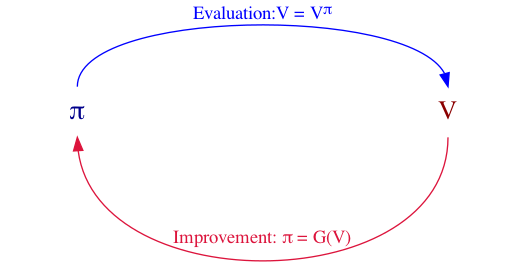
\includegraphics[width=12cm, height=8cm]{policy_iteration_loop.png}
\end{frame}

\begin{frame}
\frametitle{Convergence of Policy Iteration algorithm}

\includegraphics[width=12cm, height=8cm]{policy_iteration_convergence.png}
\end{frame}

\begin{frame}
\frametitle{Policy Iteration Convergence Theorem}
\begin{theorem}[Policy Iteration Convergence Theorem]
For a Finite MDP with $|\mathcal{N}| = m$ and $\gamma < 1$, Policy Iteration algorithm converges to the Optimal Value Function $\bvs \in \mathbb{R}^m$ along with a Deterministic Optimal Policy $\pi_D^*: \mathcal{N} \rightarrow \mathcal{A}$, no matter which Value Function $\bm{V_0} \in \mathbb{R}^m$ we start the algorithm with.
\label{eq:policy_iteration_convergence_theorem}
\end{theorem}
\end{frame}

\begin{frame}
\frametitle{Optimal Policy achieves Optimal Value Function}
\begin{theorem}
For any (discrete-time, countable-spaces, stationary) MDP:
\pause
\begin{itemize}[<+->]
\item There exists an Optimal Policy $\pi^* \in \Pi$, i.e., there exists a Policy $\pi^* \in \Pi$ such that $V^{\pi^*}(s) \geq V^{\pi}(s) \text{ for all policies  } \pi \in \Pi \mbox{ and for all states } s \in \mathcal{N}$
\item All Optimal Policies achieve the Optimal Value Function, i.e. $V^{\pi^*}(s) = V^*(s)$ for all $s \in \mathcal{N}$, for all Optimal Policies $\pi^*$
\item All Optimal Policies achieve the Optimal Action-Value Function, i.e. $Q^{\pi^*}(s,a) = Q^*(s,a)$ for all $s \in \mathcal{N}$, for all $a \in \mathcal{A}$, for all Optimal Policies $\pi^*$
\end{itemize}
\label{th:optimal-policy-achieves-optimal-value-function}
\end{theorem}
\end{frame}

\begin{frame}
\frametitle{Proof Outline}
\pause
\begin{itemize}[<+->]
\item For any Optimal Policies $\pi_1^*$ and $\pi_2^*$, $V^{\pi_1^*}(s) = V^{\pi_2^*}(s)$ for all $s \in \mathcal{N}$
\item Construct a candidate Optimal (Deterministic) Policy $\pi_D^* : \mathcal{N} \rightarrow \mathcal{A}$:
 $$\pi_D^*(s) = \argmax_{a \in \mathcal{A}} Q^*(s,a) \text{ for all } s \in \mathcal{N}$$
 \item $\pi_D^*$ achieves the Optimal Value Functions $V^*$ and $Q^*$:
 $$V^*(s) = Q^*(s,\pi_D^*(s)) \text{ for all } s \in \mathcal{N}$$
 $$V^{\pi_D^*}(s) = V^*(s) \text{ for all } s \in \mathcal{N}$$
$$Q^{\pi_D^*}(s,a) = Q^*(s,a) \text{ for all } s \in \mathcal{N}, \text{ for all } a \in \mathcal{A}$$
\item $\pi_D^*$ is an Optimal Policy:
$$V^{\pi_D^*}(s) \geq V^{\pi}(s) \text{ for all policies  } \pi \in \Pi \text{ and for all states } s \in \mathcal{N}$$
\end{itemize}
\end{frame}

\begin{frame}
\frametitle{State Space Size and Transitions Complexity}
\pause
\begin{itemize}[<+->]
\item Tabular Algorithms for State Spaces that are not too large
\item In real-world, state spaces are very large/infinite/continuous
\item {\em Curse of Dimensionality}: Size Explosion as a function of dimensions
\item {\em Curse of Modeling}: Transition Probabilities hard to model/estimate
\item Dimension-Reduction techniques, Unsupervised ML methods
\item Function Approximation of the Value Function (in ADP and RL)
\item Sampling, Sampling, Sampling ... (in ADP and RL)
\end{itemize}
\end{frame}

\begin{frame}
\frametitle{Action Space Sizes}
\pause
\begin{itemize}[<+->]
\item Large Action Spaces: Hard to represent, estimate and evaluate:
\begin{itemize}
\item Policy $\pi$
\item Action-Value Function for a policy $Q^{\pi}$
\item Optimal Action-Value Function $Q^*$
\end{itemize}
\item Large Actions Space makes it hard to calculate $\argmax_a Q(s,a)$
\item Optimization over Action Space for each non-terminal state
\item Policy Gradient a technique to deal with large action spaces
\end{itemize}
\end{frame}

\begin{frame}
\frametitle{Time-Steps Variants and Continuity}
\pause
\begin{itemize}[<+->]
\item Time-Steps: terminating ({\em episodic}) or non-terminating ({\em continuing})
\item Discounted or Undiscounted MDPs, Average-Reward MDPs
\item Continuous-time MDPs: Stochastic Processes and Stochastic Calculus
\item When States/Actions/Time all continuous, Hamilton-Jacobi-Bellman
\end{itemize}
\end{frame}

\begin{frame}
\frametitle{Partially-Observable Markov Decision Process (POMDP)}
\pause
\begin{itemize}[<+->]
\item Two different notions of {\em State}:
\begin{itemize}
\item Internal representation of the environment at each time step $t$ ($S_t^{(e)}$)
\item The agent's state at each time step $t$ (let's call it $S_t^{(a)}$)
\end{itemize}
\item We assumed $S_t^{(e)} = S_t^{(a)} (= S_t)$ and that $S_t$ is {\em fully observable}
\item A more general framework assumes agent sees {\em Observations} $O_t$
\item Agent cannot see (or infer) $S_t^{(e)}$ from history of observations
\item This more general framework is called {\em POMDP}
\item POMDP is specified with {\em Observation Space} $\mathcal{O}$ and observation probability function 
$\mathcal{Z}: \mathcal{S} \times \mathcal{A} \times \mathcal{O} \rightarrow [0, 1]$
defined as:
$$\mathcal{Z}(s', a, o) = \mathbb{P}[O_{t+1} = o | (S_{t+1}^{(e)} = s', A_t = a)]$$
\item Along with the usual transition probabilities specification $\mathcal{P}_R$
\item MDP is a special case of POMDP with $O_t = S_t^{(e)} = S_t^{(a)}$
\end{itemize}
\end{frame}

\begin{frame}
\frametitle{POMDP Framework}
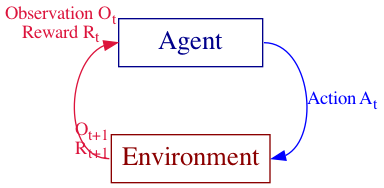
\includegraphics[width=12cm, height=8cm]{pomdp.png}
\end{frame}

\begin{frame}
\frametitle{Belief States, Tractability and Modeling}
\pause
\begin{itemize}[<+->]
\item Agent doesn't have knowledge of $S_t^{(e)}$, only of $O_t$
\item So Agent has to ``guess'' $S_t$ by maintaining {\em Belief States}
$$b(h)_t = (\mathbb{P}[S_t=s_1 | H_t = h], \mathbb{P}[S_t = s_2 | H_t = h], \ldots )$$
where history $H_t$ is all data known to agent by time $t$:
$$H_t := (O_0, R_0, A_0, O_1, R_1, A_1, \ldots, O_t, R_t)$$
\item $H_t$ satisfies Markov Property $\Rightarrow  b(h)_t$ satisfies Markov Property
\item POMDP yields (huge) MDP whose states are POMDP's belief states
\item Read-world: Model as accurate POMDP or approx as tractable MDP?
\end{itemize}
\end{frame}

\begin{frame}
\frametitle{Key Takeaways from this Chapter}
\pause
\begin{itemize}[<+->]
\item MDP Bellman Policy Equations
\item MDP Bellman Optimality Equations
\item Existence of an Optimal Policy, and of each Optimal Policy achieving the Optimal Value Function
\end{itemize}
\end{frame}


\end{document}